\begin{frame}
\frametitle{Subpass}
\begin{columns}

\column{.55\textwidth}

\begin{itemize}
\item Abbiamo un solo subpass che usa il nostro attachment
\item Durante questo subpass usiamo l'attachment come color target
\item Per questo motivo, durante questo subpass, il nostro attachment deve avere un layout adeguato
\end{itemize}

\column{.25\textwidth}

\begin{figure}[ht]
    \centering
    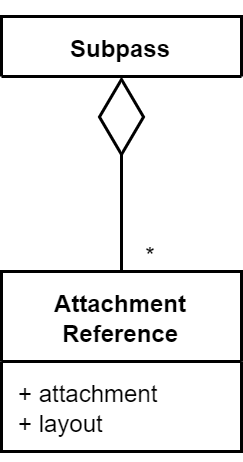
\includegraphics[scale=0.3]{images/SlidesClearWindow/Subpass.png}
\end{figure}

\end{columns}
\end{frame}
